Scopo dell'esperienza è la determinazione sperimentale dell'indice di rifrazione dell'acqua,
utilizzando la legge di Snell. Per svolgere l'esperimento è stato utilizzato un semplice setup costituito da una vaschetta di plastica trasparente con carta millimetrata visibile sul fondo, un'asta con un'altezza superiore a quella della vaschetta e una riga. L'asta è munita di un mirino mobile, che viene fissato ad una altezza prestabilita per tutta la durata dell'esperimento, allo scopo di  mantenere fissa la posizione di osservazione.

\begin{figure}[H]
	\centering
	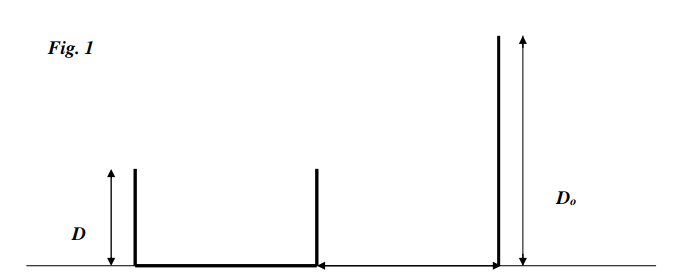
\includegraphics[width=0.75\textwidth]{./figures/Im1}
	\caption{Sezione trasversale della vaschetta, rappresentata da tre segmenti adiacenti in grassetto (di altezza $D$) e l'asta, di altezza $D_0$.}
\end{figure}

\begin{figure}[H]
	\centering
	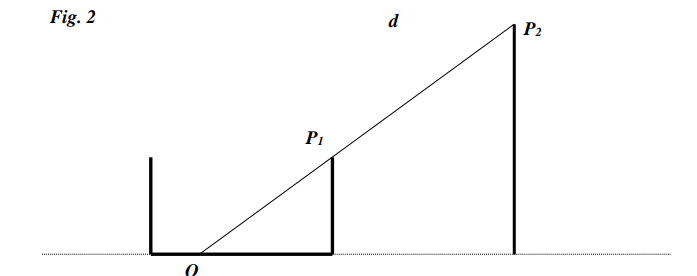
\includegraphics[width=0.75\textwidth]{./figures/Im2}
	\caption{$P_2$ è il punto fisso sull'asta da cui si effettuano le osservazioni, mentre $P_1$ è la cima della vaschetta. Quando questa è vuota, la retta $P_1P_2$ interseca il fondo nel punto $O$, che rappresenta il punto effettivamente osservato.}
\end{figure}

Fissato il punto $O$, si riempie gradualmente la vaschetta d'acqua. All'aumentare del livello $h$, osservando in direzione $P_1 P_2$, la rifrazione sposta l'immagine di $O$ in $O'$, come illustrato in Figura (3).

\begin{figure}[H]
	\centering
	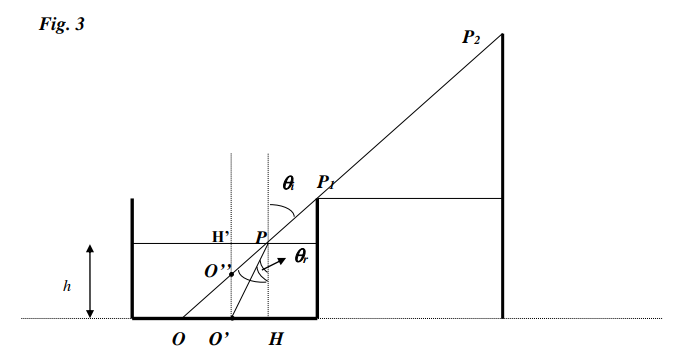
\includegraphics[width=0.75\textwidth]{./figures/Im3}
	\caption{Effetto della rifrazione dovuto alla presenza di un liquido all'interno della vaschetta, il cui livello è $H'$ e l'angolo di rifrazione $\theta_r$. In figura è anche riportato l'angolo di incidenza $\theta_i$.}
\end{figure}

La distanza $OO'$, che sarà indicata con $x$, al variare del livello dell'acqua $h$ segue un andamento lineare, in particolare: 

\begin{equation}
	x=h(\tan(\theta_i)-\tan(\theta_r))
\end{equation}

Riportando in grafico $x$ in funzione di $h$ è possibile calcolare l'angolo di rifrazione $\theta_r$ dal coefficiente angolare della retta di regressione. L'angolo di incidenza $\theta_i$ è misurabile a partire da semplici considerazioni trigonometriche. A questo punto, tramite la Legge (1), si ottiene l'indice di rifrazione.

